\documentclass[12pt]{jreport}
\usepackage[dvipdfmx]{graphicx}
\title{後期実験:マイクロプロセッサの設計と実装}
\author{電気電子工学科3年\\03210499\\高原陽太}
\date{\today}
\begin{document}
  \maketitle
  はじめに

  今回のマイクロプロセッサ実験を通して、設計から実装まで自力で行った。
  そこで今回のレポートに関しては、基本課題と応用課題に取り組むに当たって工夫した点、
  苦労した点のそれぞれについて記述して行きたいと思う。
  
  基本的なcpuの設計

  まず実験1-8日目は基本的なcpuの設計と実装を行った。構造は
  wikiの資料を参考にして作成した。
  
  工夫した箇所はストア命令を読み出す際に書き込む部分の
  指定をするための4bitのフラグを指定するためのモジュールを事前に作成したこと
  である。図1のstoreモジュールに対応している。このモジュールを作ったことにより
  データメモリへの書き込みに必要な作業を分担することができた。


  [実験結果]\\
  実装した結果は以下の通りである。
  \begin{figure}
    \centering
    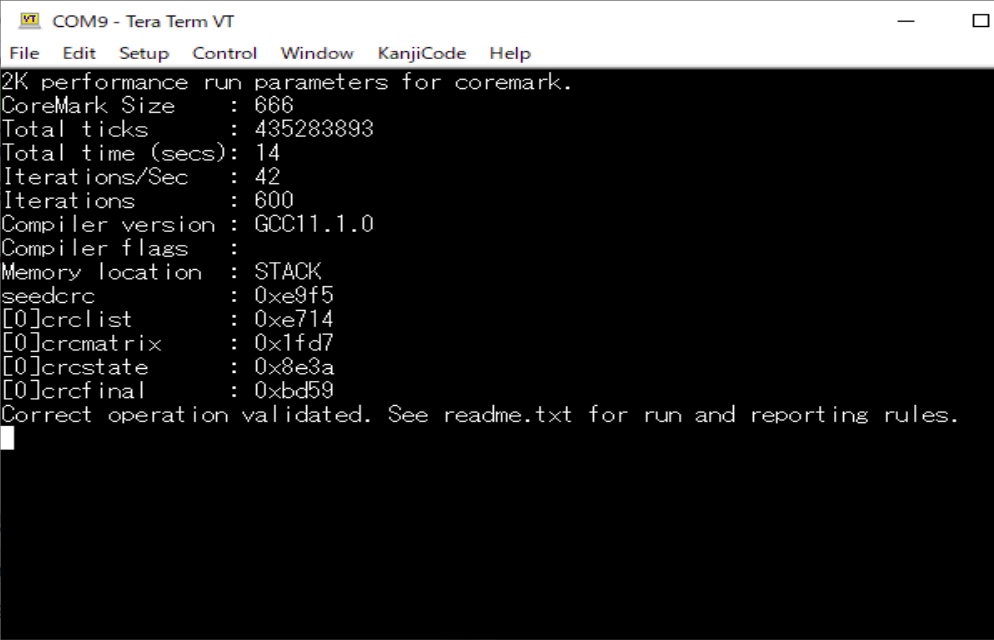
\includegraphics[width=8cm]{picture/score.png}
    \caption{最終的なCoreMarkのスコア}
  \end{figure}

  最終的なスコアは図2に示されている通り、
  \begin{equation}Iterations/Sec=42\end{equation}
  であった。これは基本課題として設計したcpuについてできるかぎり
  クリティカルパスなどを考慮し、動作周波数を$30MHz$として
  動かした際の実行結果である。

  [苦労した点]\\
  cpuを作る上で苦労した点は以下の通りである。\\
  ・ロードストア命令におけるメモリ番地の指定\\
  ・クロックの扱い\\ 
  
  まずロードストア命令におけるメモリ番地の指定についてである。
  今回のRISC-Vの仕様ではメモリのアドレシングの単位はバイトである。
  したがって、aluの演算結果として読み出されたアドレスではそのままメモリ
  中の1バイトを特定することにはならない。そこで読み込んだアドレスを
  メモリ中のデータのインデントとして利用するにはそれぞれのアドレスを
  4で割る必要があり、このことを理解するのに時間を要した。またデータ語中のバイトの並べ方が
  リトルエンディアンであるため、aluから受け取ったアドレスの下位2bitを4で割った余りについて
  ロード命令のメモリを読み出しを場合分けする必要があり、実装に苦心した。

  また、クロックを用いてメモリを制御することに関しても工夫した。今回のcpuは
  シングルプロセッサであるので1クロックでメモリに関する処理についても終了
  させる必要がある。しかし、フリップフロップにしてしまうと資源消費が大きくなってしまう。
  そのためできるだけブロックRAMの書き方にすることで資源消費量を抑えようとした。そこで
  命令メモリとデータメモリに読み出したり書き込むタイミングを別々にした。


  具体的には命令メモリの読み出しをクロックの立ち上がりで行い、データメモリに関する読み出し書き込みは
  クロックの立ち下がりで行うようにした。

  [発展課題]\\
  ・RV32Mへの対応\\
  ・クリティカルパスの短縮\\
  ・function文による記述\\

  まず、乗算器除算器の実装を行った。基本的にはdecoderとaluについて
  の書き換えのみを行った。decoderについては仕様書を見る限り25bit目の値が1かどうかで
  判別できるので、できるだけコードが簡略できるようにした。aluに関しては符号付き
  かどうかに注意しながら実装した。その際に例外的な数値などはdefine.vhにまとめて記載することで
  間違いを減らすようにした。\\
  RV32Mへの対応に関して最も苦労したのは実行時間増加に伴うクリティカルパスの
  延長であった。乗算器が非常に遅いためそれによって今まで動いていた動作周波数で稼働しなくなってしまった。
  そのため遅延しても稼働するようにクリティカルパスの短縮とfunction文による記述という
  工夫を行った。
  \begin{figure}
    \centering
    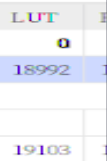
\includegraphics[width=5cm]{picture/lut1.png}
    \caption{最初の消費資源量}
    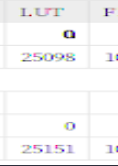
\includegraphics[width=5cm]{picture/lut2.png}
    \caption{RV32M後の消費資源量}
  \end{figure}
  
  また乗算器除算器を取り入れたことにより消費資源量も増えてしまった。これも
  回路のコードに余分な箇所、重複している箇所があることに起因していると考えた。

  下図がクリティカルパスである。大まかに見ると図のcpuの赤線部分のような
  経路がクリティカルパスになっていることが分かる。データメモリから読み出してくる
  ロード命令が一番遅いと考えた。そこでできるだけデータメモリに関する処理を簡単にすることを考えた。
  考えたのがfunction文による記述である。自分のコードを見返す限り、データメモリだけでなくdecoderやalu
  についてもalways文の中で巨大なcase文を用いて記述してしまったことで回路が複雑化してしまい、Vivadoが最適化をできなくなってしまったの
  ではないかと考えた。\\
   実際にfunction文で記述し直したところ、decoderとaluに関しては
  記述量を半分以下にまで減らすことができた。\\
  \begin{figure}
    \centering
    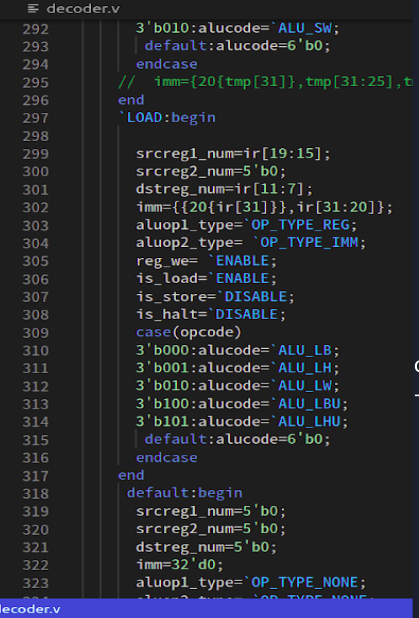
\includegraphics[width=5cm]{picture/deco.png}
    \caption{当初のdecoderのコード}
    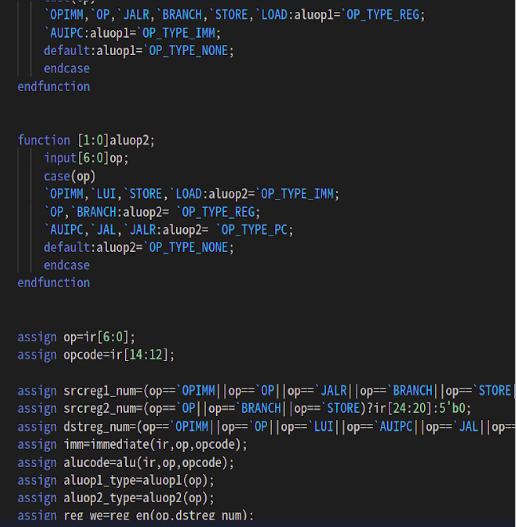
\includegraphics[width=7cm]{picture/deco2.png}
    \caption{簡略化したdecoderのコードs}
  \end{figure}
  
  しかしregとして存在しているメモリを参照する
  必要があるデータメモリをfunction文で書くことができなかった。function文
  と同様の機能を導入するにはalways(*)でも記述することができるがそれだとブロックRAMにならないためデータメモリに関しては
  always文とcase文を用いて記述せざるを得なかった。\\
  データメモリに関しては上記のようにストアのフラグを立てる箇所を分離するなどして
  できるだけ処理を減らすことでクリティカルパスの短縮を試みた。
  



  \begin{figure}
    \centering
    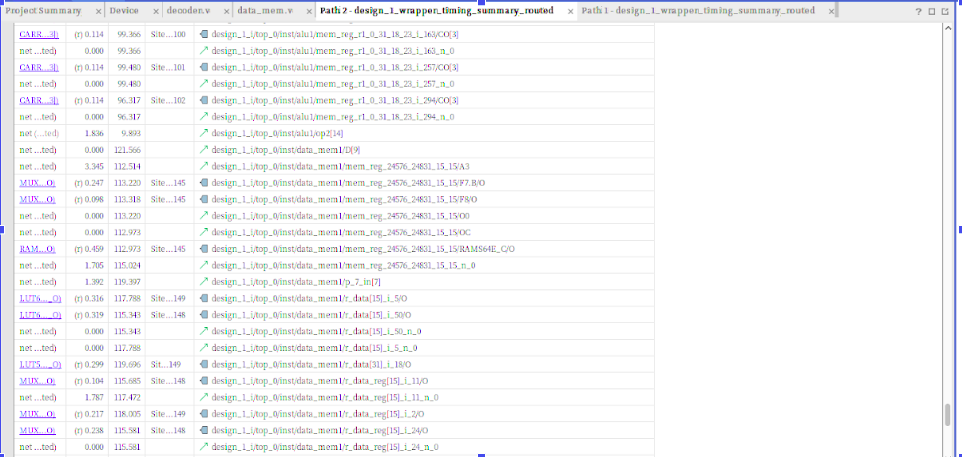
\includegraphics[width=10cm]{picture/cri.png}
    \caption{クリティカルパス}
  \end{figure}





  \begin{figure}
    \centering
    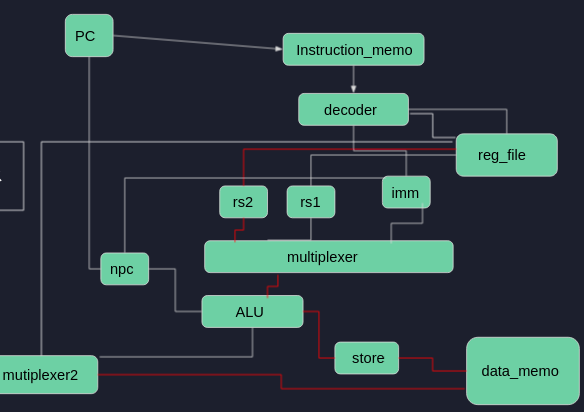
\includegraphics[width=8cm]{picture/cpu.png}
    \caption{cpuの図}
  \end{figure}
  
\end{document}
